\documentclass{article}

% content/resources/templates/preamble.tex
\usepackage[margin=0.6in]{geometry}
\author{Milav Dabgar}
\usepackage{amsmath,amssymb,amsthm}
\usepackage{booktabs}
\usepackage{multirow}
\usepackage{xcolor}
\usepackage{tcolorbox}
\tcbuselibrary{breakable,skins}
\usepackage[colorlinks=true,linkcolor=blue]{hyperref}
\usepackage{titlesec}
\usepackage{enumitem}
\usepackage{tikz}
\usepackage{pgfplots}
\usepackage{circuitikz}
\usepackage[version=4]{mhchem}
\usepackage{longtable}
\usepackage{array}
\usepackage{float}
\usepackage{caption}
\usepackage{listings}

\lstset{
  basicstyle=\small\ttfamily,
  breaklines=true,
  breakatwhitespace=false,
  postbreak=\mbox{\textcolor{red}{$\hookrightarrow$}\space},
  float=false,
  numbers=left,
  numberstyle=\tiny\color{gray},
  numbersep=10pt,
  xleftmargin=2em,
  keywordstyle=\color{blue},
  commentstyle=\color{green!60!black},
  stringstyle=\color{purple},
  backgroundcolor=\color{gray!5},
  showstringspaces=false,
  tabsize=2,
  captionpos=b,
  keepspaces=true,
  columns=flexible
}

\pgfplotsset{compat=1.18}
\usetikzlibrary{shapes,arrows,positioning,calc,patterns,decorations.pathmorphing,decorations.markings,arrows.meta}

% Color scheme
\definecolor{headcolor}{RGB}{0,102,204}
\definecolor{keycolor}{RGB}{220,20,60}
\definecolor{solutioncolor}{RGB}{34,139,34}
\definecolor{mnemoniccolor}{RGB}{148,0,211}
\definecolor{codecolor}{RGB}{0,0,100}

% Spacing
\setlength{\parskip}{3pt}
\setlist[itemize]{nosep}
\setlist[enumerate]{nosep}

% Title formatting
\titleformat{\section}{\Large\bfseries\color{headcolor}}{\thesection}{1em}{}
\titleformat{\subsection}{\large\bfseries\color{headcolor}}{\thesubsection}{1em}{}

% Pandoc tightlist compatibility
\providecommand{\tightlist}{%
  \setlength{\itemsep}{0pt}\setlength{\parskip}{0pt}}

% Pandoc longtable compatibility
\newcounter{none}
\def\thenone{}


% content/resources/templates/english-boxes.tex

% Custom environments
\newtcolorbox{solutionbox}{
 breakable,
 enhanced,
 colback=solutioncolor!5!white,
 colframe=solutioncolor!75!black,
 fonttitle=\bfseries,
 title=Solution
}

\newtcolorbox{solutionboxnobreak}{
 colback=solutioncolor!5!white,
 colframe=solutioncolor!75!black,
 fonttitle=\bfseries,
 title=Solution
}

\newtcolorbox{keyformula}{
 breakable,
 enhanced,
 colback=keycolor!5!white,
 colframe=keycolor!75!black,
 fonttitle=\bfseries,
 title=Key Formula
}

\newtcolorbox{mnemonicboxenv}{
 breakable,
 enhanced,
 colback=mnemoniccolor!5!white,
 colframe=mnemoniccolor!75!black,
 fonttitle=\bfseries,
 title=Mnemonic
}

\newcommand{\mnemonicbox}[1]{%
  \begin{mnemonicboxenv}
    #1
  \end{mnemonicboxenv}
}


% Custom commands for GTU solutions
% This file defines semantic commands for consistent formatting

% Question command with automatic formatting
\newcommand{\question}[2]{%
  \section*{Question #1}%
  \textbf{#2}%
}

% OR question variant
\newcommand{\questionor}[2]{%
  \section*{Question #1 OR}%
  \textbf{#2}%
}

% Proper table environment with caption
\newenvironment{answertable}[1]{%
  \begin{table}[htbp]
  \centering
  \caption{#1}
}{%
  \end{table}
}

% Proper figure environment for diagrams
\newenvironment{answerdiagram}[1]{%
  \begin{figure}[htbp]
  \centering
  \caption{#1}
}{%
  \end{figure}
}

% Semantic markup for key terms
\newcommand{\keyword}[1]{\textbf{#1}}
\newcommand{\code}[1]{\texttt{#1}}
\newcommand{\classname}[1]{\texttt{#1}}
\newcommand{\methodname}[1]{\texttt{#1}}

% Proper quotation marks
\newcommand{\mnemonic}[1]{``#1''}


\title{Electronics Devices \& Circuits (1323202) - Winter 2023 Solution}
\date{January 24, 2024}

\begin{document}
\maketitle


\questionmarks{1(a)}{3}{Explain the concept of dc load line with the help of neat diagram.}

\begin{solutionbox}
DC load line is a straight line on output characteristics that shows all possible operating points of a transistor.

\textbf{Diagram:}

\begin{center}
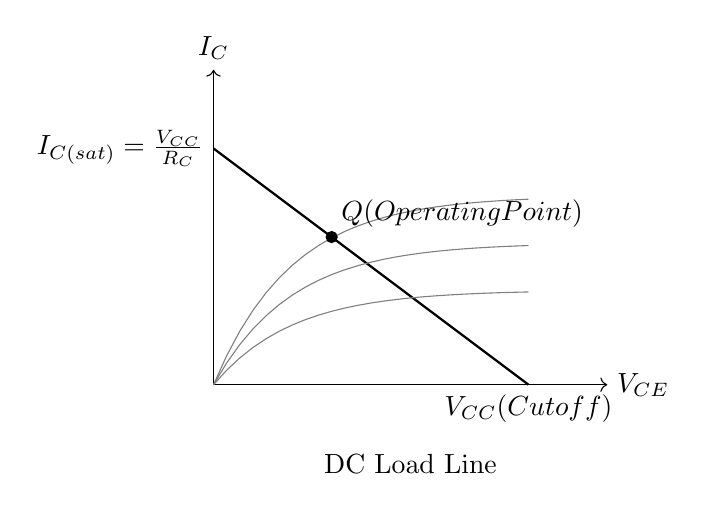
\begin{tikzpicture}[scale=1]
    % Axes
    \draw[->] (0,0) -- (5,0) node[right] {$V_{CE}$};
    \draw[->] (0,0) -- (0,4) node[above] {$I_C$};
    
    % Load Line
    \draw[thick] (0,3) node[left] {$I_{C(sat)} = \frac{V_{CC}}{R_C}$} -- (4,0) node[below] {$V_{CC} (Cutoff)$};
    
    % Curves (optional but good for context)
    \draw[gray, domain=0:4] plot (\x, {3*(1-exp(-\x))*0.8});
    \draw[gray, domain=0:4] plot (\x, {3*(1-exp(-\x))*0.6});
    \draw[gray, domain=0:4] plot (\x, {3*(1-exp(-\x))*0.4});
    
    % Q-point
    \filldraw (1.5, 1.875) circle (2pt) node[above right] {$Q (Operating Point)$};
    
    \node at (2.5, -1) {DC Load Line};
\end{tikzpicture}
\end{center}

\begin{itemize}
    \item \textbf{Collector saturation current}: When $V_{CE} = 0$, $I_C = V_{CC}/R_C$
    \item \textbf{Cutoff voltage}: When $I_C = 0$, $V_{CE} = V_{CC}$
    \item \textbf{Q-point}: Operating point along load line
\end{itemize}

\begin{mnemonicbox}
"LEVEL" - "Load line Establishes Voltage and current for Every Load condition"
\end{mnemonicbox}
\end{solutionbox}

\questionmarks{1(b)}{4}{Explain thermal runaway in detail.}

\begin{solutionbox}
Thermal runaway is a condition where heat causes transistor's collector current to increase, which generates more heat, leading to destruction.

\textbf{Diagram:}

\begin{center}
\begin{tikzpicture}[gtu block]
    \node [draw, rectangle] (temp1) {Temperature Increases};
    \node [draw, rectangle, below=0.8cm of temp1] (leak) {Leakage Current Increases};
    \node [draw, rectangle, below=0.8cm of leak] (ic) {Collector Current Increases};
    \node [draw, rectangle, below=0.8cm of ic] (power) {More Power Dissipation};
    \node [draw, rectangle, below=0.8cm of power] (temp2) {Further Temperature Rise};
    
    \draw [gtu arrow] (temp1) -- (leak);
    \draw [gtu arrow] (leak) -- (ic);
    \draw [gtu arrow] (ic) -- (power);
    \draw [gtu arrow] (power) -- (temp2);
    \draw [gtu arrow] (temp2.east) to[out=0,in=0] (temp1.east);
\end{tikzpicture}
\end{center}

\begin{itemize}
    \item \textbf{Heat generation}: Power dissipation = $V_{CE} \times I_C$
    \item \textbf{Critical effect}: Increased junction temperature decreases $V_{BE}$
    \item \textbf{Prevention}: Heat sinks, thermal stabilization circuits, proper biasing
    \item \textbf{Danger}: Can destroy transistor if not controlled
\end{itemize}

\begin{mnemonicbox}
"HEAT" - "Higher Emission Amplifies Temperature"
\end{mnemonicbox}
\end{solutionbox}

\questionmarks{1(c)}{7}{Draw the circuit diagram and frequency response of a two stage R-C coupled amplifier. Explain the importance of each component.}

\begin{solutionbox}
R-C coupled amplifier uses capacitors to connect multiple transistor stages for higher gain.

\textbf{Circuit Diagram:}

\begin{center}
\begin{circuitikz}[american, scale=0.9, transform shape]
    % Stage 1
    \draw (0,0) node[ground] {} to[R, l=$R_{E1}$] (0,1) to[Tnpn, n=Q1] (0,3) to[R, l=$R_{C1}$] (0,5) -- (0,6) node[vcc] {$V_{CC}$};
    \draw (Q1.B) -- (-1.5, 1.85); 
    \draw (-1.5, 6) to[R, l=$R_1$] (-1.5, 1.85) to[R, l=$R_2$] (-1.5, 0) node[ground] {};
    \draw (-3.5, 1.85) to[C, l=$C_{in}$] (-1.5, 1.85);
    \draw (-3.5, 1.85) node[left] {$V_{in}$};
    \draw (0,1) -- (1,1) to[C, l=$C_{E1}$] (1,0) node[ground] {};
    
    % Coupling
    \draw (0,3) to[C, l=$C_C$] (3,3) -- (3, 1.85);
    
    % Stage 2
    \draw (4.5,0) node[ground] {} to[R, l=$R_{E2}$] (4.5,1) to[Tnpn, n=Q2] (4.5,3) to[R, l=$R_{C2}$] (4.5,5) -- (4.5,6) -- (0,6);
    \draw (Q2.B) -- (3, 1.85);
    \draw (3, 6) to[R, l=$R_3$] (3, 1.85) to[R, l=$R_4$] (3, 0) node[ground] {};
    \draw (4.5,1) -- (5.5,1) to[C, l=$C_{E2}$] (5.5,0) node[ground] {};
    
    % Output
    \draw (4.5,3) to[C, l=$C_{out}$] (6.5,3) node[right] {$V_{out}$};
    
    \draw (-1.5, 6) -- (0,6);
    \draw (3,6) -- (4.5,6);
\end{circuitikz}
\end{center}

\textbf{Frequency Response:}

\begin{center}
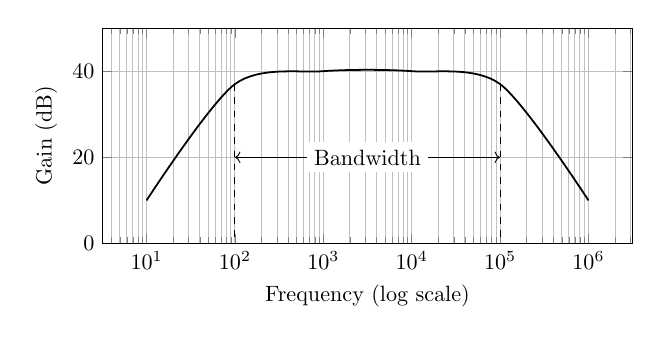
\begin{tikzpicture}[scale=0.8]
    \begin{axis}[
        xlabel={Frequency (log scale)},
        ylabel={Gain (dB)},
        xmode=log,
        ymin=0, ymax=50,
        grid=both,
        width=10cm, height=5cm
    ]
    \addplot[smooth, thick] coordinates {
        (10, 10) (100, 37) (1000, 40) (10000, 40) (100000, 37) (1000000, 10)
    };
    \draw[dashed] (100, 37) -- (100, 0) node[below] {$f_L$};
    \draw[dashed] (100000, 37) -- (100000, 0) node[below] {$f_H$};
    \draw[<->] (100, 20) -- (100000, 20) node[midway, fill=white] {Bandwidth};
    \end{axis}
\end{tikzpicture}
\end{center}

\begin{itemize}
    \item \textbf{Coupling capacitors ($C_C$)}: Block DC, allow AC signal transfer between stages
    \item \textbf{Biasing resistors ($R_1, R_2$)}: Establish proper Q-point for transistor operation
    \item \textbf{Bypass capacitors ($C_E$)}: Prevent gain reduction from negative feedback across $R_E$
    \item \textbf{Bandwidth}: Range between low ($f_L$) and high ($f_H$) cutoff frequencies
\end{itemize}

\begin{mnemonicbox}
"CARS" - "Coupling capacitors Allow Resistance Separation"
\end{mnemonicbox}
\end{solutionbox}

\vspace{0.5em}\centerline{\textbf{OR}}\questionmarks{1(c)}{7}{Compare negative and positive feedback in amplifier.}

\begin{solutionbox}
Feedback systems return a portion of output to the input with different effects based on polarity.

\begin{center}
\captionof{table}{Comparison of Feedback Types}
\begin{tabulary}{\textwidth}{|L|L|L|}
\hline
\textbf{Parameter} & \textbf{Negative Feedback} & \textbf{Positive Feedback} \\
\hline
Gain & Decreases & Increases \\
\hline
Bandwidth & Increases & Decreases \\
\hline
Stability & Improves & Decreases \\
\hline
Distortion & Reduces & Increases \\
\hline
Noise & Reduces & Amplifies \\
\hline
Input/Output Impedance & Can be controlled & Unpredictable \\
\hline
Applications & Amplifiers, regulators & Oscillators, Schmitt triggers \\
\hline
\end{tabulary}
\end{center}

\begin{itemize}
    \item \textbf{Negative feedback}: Output is out of phase with input (180° shifted)
    \item \textbf{Positive feedback}: Output is in phase with input (0° shifted)
    \item \textbf{Barkhausen criteria}: Positive feedback with unity gain creates oscillation
\end{itemize}

\begin{mnemonicbox}
"SIGN" - "Stability Increases with Gain Negation"
\end{mnemonicbox}
\end{solutionbox}
\questionmarks{2(a)}{3}{State and explain Barkhausen's criteria for oscillations.}

\begin{solutionbox}
Barkhausen's criteria define conditions for sustained oscillations in a feedback system.

\textbf{Diagram:}

\begin{center}
\begin{tikzpicture}[gtu block]
    \node [draw, rectangle] (amp) {Amplifier ($A$)};
    \node [draw, rectangle, below=1cm of amp] (beta) {Feedback Network ($\beta$)};
    \node [left=1cm of amp] (in) {};
    \node [right=1cm of amp] (out) {};

    \draw [gtu arrow] (in) -- node[above] {$V_{in}=0$} (amp);
    \draw [gtu arrow] (amp) -- node[above] {$V_{out}$} (out);
    \draw [gtu arrow] (amp.east) -- ++(0.5,0) |- (beta.east);
    \draw [gtu arrow] (beta.west) -| (amp.west);
    
    \node [right, align=left] at (4,0) {Conditions:\\1. Loop Gain $|A\beta| = 1$\\2. Phase Shift $\angle A\beta = 0^\circ$ or $360^\circ$};
\end{tikzpicture}
\end{center}

\begin{itemize}
    \item \textbf{Gain condition}: Loop gain ($A\times\beta$) must equal 1 (unity)
    \item \textbf{Phase condition}: Total phase shift around the loop must be $0^\circ$ or $360^\circ$
    \item \textbf{Practical implementation}: Initial loop gain $> 1$ to start, then stabilizes at 1 due to nonlinearity
\end{itemize}

\begin{mnemonicbox}
"LOOP" - "Loop's Overall Output Phase"
\end{mnemonicbox}
\end{solutionbox}

\questionmarks{2(b)}{4}{Compare Fixed bias, Collector to base bias \& Voltage divider bias methods.}

\begin{solutionbox}
Different biasing techniques provide varying degrees of stability and temperature compensation.

\begin{center}
\captionof{table}{Comparison of Biasing Methods}
\begin{tabulary}{\textwidth}{|L|L|L|L|}
\hline
\textbf{Parameter} & \textbf{Fixed Bias} & \textbf{Collector-Base Bias} & \textbf{Voltage Divider Bias} \\
\hline
Stability & Poor & Better & Excellent \\
\hline
Circuit Complexity & Simple & Medium & Complex \\
\hline
Temp Stability & Poor & Medium & Good \\
\hline
Components & 1 Resistor & 1 Resistor & 3-4 Resistors \\
\hline
Stability Factor (S) & High (Unstable) & Medium & Low (Stable) \\
\hline
\end{tabulary}
\end{center}

\begin{itemize}
    \item \textbf{Fixed bias}: Single resistor from base to $V_{CC}$
    \item \textbf{Collector-base bias}: Feedback resistor from collector to base provides negative feedback
    \item \textbf{Voltage divider}: Two resistors create stable reference voltage independent of $\beta$
\end{itemize}

\begin{mnemonicbox}
"STORM" - "Stability Through Optimized Resistor Methods"
\end{mnemonicbox}
\end{solutionbox}

\questionmarks{2(c)}{7}{Write short note on Hartley oscillator.}

\begin{solutionbox}
Hartley oscillator is an LC oscillator with a tapped inductor for feedback.

\textbf{Circuit Diagram:}

\begin{center}
\begin{circuitikz}[american, scale=0.9, transform shape]
    \draw (0,0) node[ground] {} to[R, l=$R_E$] (0,1) to[Tnpn, n=Q1] (0,3) to[L, l=$RFC$] (0,5) -- (0,6) node[vcc] {$V_{CC}$};
    \draw (0,1) -- (1,1) to[C, l=$C_E$] (1,0) node[ground] {};
    
    % Biasing
    \draw (-1.5, 6) to[R, l=$R_1$] (-1.5, 1.85) to[R, l=$R_2$] (-1.5, 0) node[ground] {};
    \draw (-1.5, 6) -- (0,6);
    \draw (Q1.B) -- (-1.5, 1.85);
    
    % Tank Circuit
    \draw (3,5) to[C, l=$C_{out}$] (0,3); 
    \draw (3,5) -- (5,5) to[L, l=$L_1$] (5,3) to[L, l=$L_2$] (5,1) -- (5,0) node[ground] {};
    \draw (5,3) -- (6,3) node[ground] {}; % Tap to ground (Common Emitter config, though often tank is different)
    % Wait, typical Hartley has tap grounded for AC? Or Tap is input?
    % Let's draw standard Hartley: L1+L2 parallel with C. Tap connects to Emitter or Ground.
    % Common Emitter Hartley: Tank in Collector. Feedback to Base.
    % Let's refine:
    % Tank: L1+L2 || C.
    % Output taken from L1/L2 junction? No.
    % Feedback: From tank to Base.
    % Correct verify: Hartley has Tapped Inductor.
    
    % Redrawing Tank properly
    \draw (2.5, 0) node[ground] {} to[C, l=$C$] (2.5, 4) -- (4.5, 4);
    \draw (4.5, 4) to[L, l=$L_1$] (4.5, 2) to[L, l=$L_2$] (4.5, 0) -- (2.5, 0);
    \draw (4.5, 2) node[ground] {}; % Center tap grounded
    
    % Connections
    \draw (0,3) -- (0,4) to[C, l=$C_{c2}$] (2.5,4); % Collector to Tank Top
    \draw (Q1.B) -- (-2, 1.85) to[C, l=$C_{c1}$] (-2, 0) -- (4.5, 0); % Base to Tank Bottom (Feedback) - wait, this is tricky layout
    % Simpler layout:
\end{circuitikz}

\begin{circuitikz}[american, scale=0.9, transform shape]
    % Transistor
    \draw (0,0) node[ground] {} to[R, l=$R_E$] (0,1) to[Tnpn, n=Q1] (0,3) to[L, l=$RFC$] (0,5) -- (0,6) node[vcc] {$V_{CC}$};
    \draw (0,1) -- (1,1) to[C, l=$C_E$] (1,0) node[ground] {};
    
    % Biasing
    \draw (-1.5, 6) to[R, l=$R_1$] (-1.5, 1.85) -- (Q1.B);
    \draw (-1.5, 1.85) to[R, l=$R_2$] (-1.5, 0) node[ground] {};
    \draw (-1.5, 6) -- (0,6);
    
    % Tank Circuit
    \draw (3, 4) to[C, l=$C$] (3, 0);
    \draw (4.5, 4) to[L, l=$L_1$] (4.5, 2) node[ground] {} to[L, l=$L_2$] (4.5, 0);
    \draw (3,4) -- (4.5,4);
    \draw (3,0) -- (4.5,0);
    
    % Coupling
    \draw (0,3) -- (0,4) to[C, l=$C_C$] (3,4); % Collector to Tank
    \draw (-1.5, 1.85) -- (-2.5, 1.85) to[C, l=$C_{in}$] (-2.5, 0) -- (3,0); % Feedback to Base
\end{circuitikz}
\end{center}

\begin{itemize}
    \item \textbf{Circuit components}: Amplifier (CE Mode), Tank Circuit ($L_1, L_2, C$)
    \item \textbf{Frequency formula}: $f = \frac{1}{2\pi\sqrt{L_{eq}C}}$ where $L_{eq} = L_1 + L_2$
    \item \textbf{Feedback}: Voltage across $L_2$ is fed back to base ($180^\circ$ phase shift by tank + $180^\circ$ by amp = $360^\circ$)
    \item \textbf{Applications}: RF signal generators, radio receivers
\end{itemize}

\begin{mnemonicbox}
"TILC" - "Tapped Inductor with LC Circuit"
\end{mnemonicbox}
\end{solutionbox}

\vspace{0.5em}\centerline{\textbf{OR}}\questionmarks{2(a)}{3}{Explain working of transistor as a switch.}

\begin{solutionbox}
Transistor switches between cutoff (OFF) and saturation (ON) regions for digital applications.

\textbf{Diagram:}

\begin{center}
\begin{tikzpicture}[gtu block]
    \node [draw, rectangle] (in) {Input};
    \node [draw, diamond, right=1cm of in] (trans) {Transistor};
    \node [draw, rectangle, right=1cm of trans] (out) {Output};
    
    \draw [gtu arrow] (in) -- node[above] {High} (trans);
    \draw [gtu arrow] (trans) -- node[above] {Low (ON)} (out);
    
    \node [below=0.5cm of trans] (state) {State};
    \draw [dashed] (trans) -- (state);
\end{tikzpicture}
\end{center}

\begin{itemize}
    \item \textbf{Cutoff region}: $V_{BE} < 0.7V$, acts as open switch, $V_{CE} \approx V_{CC}$ (Output High)
    \item \textbf{Saturation region}: $V_{BE} > 0.7V$, acts as closed switch, $V_{CE} \approx 0.2V$ (Output Low)
    \item \textbf{Switching time}: Limited by junction capacitance
\end{itemize}

\begin{mnemonicbox}
"COPS" - "Cutoff-On-Produces Switching"
\end{mnemonicbox}
\end{solutionbox}

\questionmarks{2(b)}{4}{Define heat sink. List types of heat sink and give its applications.}

\begin{solutionbox}
Heat sink is a thermal conductor that transfers heat away from electronic components to prevent overheating.

\textbf{Diagram:}

\begin{center}
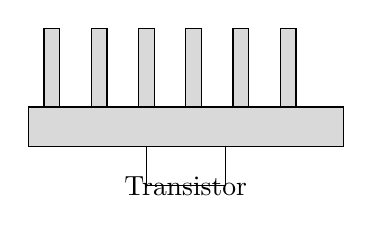
\begin{tikzpicture}
    % Simple finned heat sink
    \draw[fill=gray!30] (0,0) rectangle (4, 0.5); % Base
    \foreach \x in {0.2, 0.8, ..., 3.8}
        \draw[fill=gray!30] (\x, 0.5) rectangle (\x+0.2, 1.5); % Fins
    \node at (2, -0.5) {Transistor};
    \draw (1.5, -0.5) rectangle (2.5, 0);
\end{tikzpicture}
\end{center}

\textbf{Types of Heat Sinks:}

\begin{center}
\captionof{table}{Heat Sink Types and Applications}
\begin{tabulary}{\textwidth}{|L|L|L|}
\hline
\textbf{Type} & \textbf{Description} & \textbf{Application} \\
\hline
Passive & No moving parts, natural convection & Low-power devices \\
\hline
Active & With fans or pumps & High-power amplifiers, CPUs \\
\hline
Liquid-cooled & Uses fluid for heat transfer & Supercomputers, high-end PCs \\
\hline
Finned & Multiple fins increase surface area & Power transistors \\
\hline
\end{tabulary}
\end{center}

\begin{mnemonicbox}
"COOL" - "Conducting Out Of Local heat"
\end{mnemonicbox}
\end{solutionbox}

\questionmarks{2(c)}{7}{Explain advantages and disadvantages of negative feedback in amplifiers in detail.}

\begin{solutionbox}
Negative feedback returns a portion of output signal to input with opposite phase to improve performance stability.

\textbf{Feedback Block Diagram:}

\begin{center}
\begin{tikzpicture}[gtu block]
    \node [draw, circle] (sum) {$\Sigma$};
    \node [draw, rectangle, right=1cm of sum] (amp) {$A$};
    \node [draw, rectangle, below=1cm of amp] (beta) {$\beta$};
    \node [left=1cm of sum] (in) {$V_{in}$};
    \node [right=1cm of amp] (out) {$V_{out}$};

    \draw [gtu arrow] (in) -- node[above] {+} (sum);
    \draw [gtu arrow] (sum) -- (amp);
    \draw [gtu arrow] (amp) -- (out);
    \draw [gtu arrow] (amp.east) -- ++(0.5,0) |- (beta.east);
    \draw [gtu arrow] (beta.west) -| node[left] {-} (sum.south);
\end{tikzpicture}
\end{center}

\begin{center}
\captionof{table}{Pros and Cons of Negative Feedback}
\begin{tabulary}{\textwidth}{|L|L|}
\hline
\textbf{Advantages} & \textbf{Disadvantages} \\
\hline
Stabilizes gain against parameter changes & Reduces overall gain \\
\hline
Increases bandwidth & Requires more components \\
\hline
Reduces non-linear distortion & More power consumption in feedback circuit \\
\hline
Decreases noise & Complexity of design \\
\hline
Controls Input/Output Impedance & Potential for oscillation if phase margin low \\
\hline
\end{tabulary}
\end{center}

\begin{mnemonicbox}
"STABLE" - "Stabilized Transmission And Bandwidth with Less Error"
\end{mnemonicbox}
\end{solutionbox}
\questionmarks{3(a)}{3}{Draw symbol of SCR and explain working of SCR.}

\begin{solutionbox}
Silicon Controlled Rectifier (SCR) is a four-layer PNPN device with three terminals.

\textbf{Symbol:}

\begin{center}
\begin{circuitikz}[american, scale=1.2, transform shape]
    \draw (0,0) to[Thyristor, name=SCR] (0, 2);
    \node[above] at (0,2) {Anode (A)};
    \node[below] at (0,0) {Cathode (K)};
    \node[right] at (SCR.gate) {Gate (G)};
\end{circuitikz}
\end{center}

\begin{itemize}
    \item \textbf{Structure}: P-N-P-N four-layer semiconductor device
    \item \textbf{Operation}: Remains OFF until gate triggered, then conducts until current falls below holding value
    \item \textbf{Terminals}: Anode (A), Cathode (K), Gate (G)
\end{itemize}

\begin{mnemonicbox}
"AGK" - "Anode-Gate controls Kathode current"
\end{mnemonicbox}
\end{solutionbox}

\questionmarks{3(b)}{4}{Explain two transistor analogy of SCR with circuit diagram.}

\begin{solutionbox}
SCR can be represented as interconnected PNP and NPN transistors sharing semiconductor layers.

\textbf{Circuit Diagram:}

\begin{center}
\begin{circuitikz}[american, scale=1.0, transform shape]
    % PNP Transistor (Upper)
    \draw (2,4) node[above] {Anode} to[Tpnp, n=Q1] (2,2);
    
    % NPN Transistor (Lower)
    \draw (1,0) node[below] {Cathode} to[Tnpn, mirror, n=Q2] (1,2);
    
    % Connections
    \draw (Q1.C) -- (1,2) -- (Q2.B); % PNP Collector to NPN Base
    \draw (Q2.C) -- (2,2) -- (Q1.B); % NPN Collector to PNP Base
    
    % Gate
    \draw (Q2.B) -- (0, 0.85) node[left] {Gate};
    
    % Nodes
    \node[right] at (Q1.E) {Q1 (PNP)};
    \node[left] at (Q2.E) {Q2 (NPN)};
\end{circuitikz}
\end{center}

\begin{itemize}
    \item \textbf{PNP section}: Upper transistor with collector connected to NPN base
    \item \textbf{NPN section}: Lower transistor with collector connected to PNP base
    \item \textbf{Regenerative Feedback}: Collector current of Q1 feeds Base of Q2; Collector current of Q2 feeds Base of Q1. Once triggered, the loop sustains standard conduction.
\end{itemize}

\begin{mnemonicbox}
"PNPN" - "Positive-Negative-Positive-Negative layers"
\end{mnemonicbox}
\end{solutionbox}

\questionmarks{3(c)}{7}{Explain the working of TRIAC based fan regulator with circuit diagram.}

\begin{solutionbox}
TRIAC-based fan regulator controls AC power delivered to the load through phase control.

\textbf{Circuit Diagram:}

\begin{center}
\begin{circuitikz}[american, scale=1.0, transform shape]
    \draw (0,4) node[left] {AC Live} to[short, o-] (1,4) -- (3,4) -- (5,4);
    
    % Load
    \draw (5,4) to[lamp, l=Fan/Load] (5,2) to[Triac, n=T1, mirror] (5,0) -- (0,0) node[left] {AC Neutral} node[short, o] {};
    
    % Trigger Circuit
    \draw (1,4) to[R, l=$R_1$] (1,2.5) to[vR, l=$R_2 (Speed)$] (1,1) -- (3,1);
    \draw (3,1) to[C, l=$C_1$] (3,0) node[ground] {}; % Wait, not ground, remote neutral.
    \draw (3,0) -- (5,0); % Connect to neutral line
    
    % DIAC
    \draw (3,1) -- (3,2) to[generic, l=DIAC] (T1.gate);
    
    \node[right] at (T1) {TRIAC};
\end{circuitikz}
\end{center}

\begin{itemize}
    \item \textbf{Phase control}: Varies firing angle of TRIAC to control effective RMS voltage
    \item \textbf{Diac}: Provides bidirectional triggering pulse for TRIAC
    \item \textbf{RC timing circuit}: $R_1, R_2, C_1$ determine the delay angle; Changing $R_2$ changes speed
    \item \textbf{Operation}: When capacitor voltage reaches DIAC breakover, TRIAC fires
\end{itemize}

\begin{mnemonicbox}
"TRIAC" - "Triggered Response In AC Circuits"
\end{mnemonicbox}
\end{solutionbox}

\vspace{0.5em}\centerline{\textbf{OR}}\questionmarks{3(a)}{3}{Draw V-I characteristics of DIAC and TRIAC.}

\begin{solutionbox}
DIACs and TRIACs are bidirectional devices with symmetrical forward and reverse characteristics.

\textbf{DIAC Characteristics:}
\begin{center}
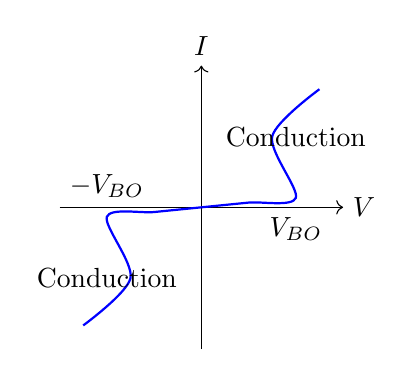
\begin{tikzpicture}[scale=0.6]
    \draw[->] (-3,0) -- (3,0) node[right] {$V$};
    \draw[->] (0,-3) -- (0,3) node[above] {$I$};
    \draw[thick, blue] plot [smooth] coordinates {(0,0) (1,0.1) (2,0.2) (1.5,1.5) (2.5,2.5)}; % Breakover and neg resistance roughly
    \draw[thick, blue] plot [smooth] coordinates {(0,0) (-1,-0.1) (-2,-0.2) (-1.5,-1.5) (-2.5,-2.5)};
    \node at (2, 1.5) {Conduction};
    \node at (-2, -1.5) {Conduction};
    \node[below] at (2,0) {$V_{BO}$};
    \node[above] at (-2,0) {$-V_{BO}$};
\end{tikzpicture}
\end{center}

\textbf{TRIAC Characteristics:}
\begin{center}
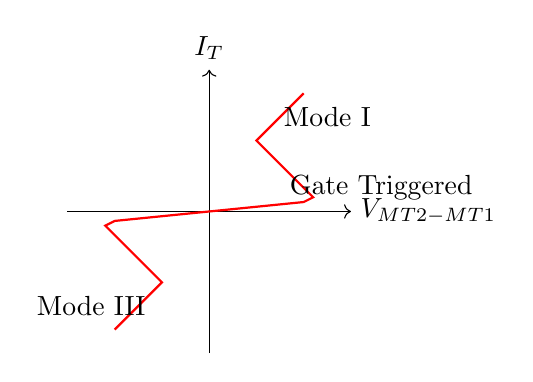
\begin{tikzpicture}[scale=0.6]
    \draw[->] (-3,0) -- (3,0) node[right] {$V_{MT2-MT1}$};
    \draw[->] (0,-3) -- (0,3) node[above] {$I_T$};
    % Quadrant 1
    \draw[thick, red] plot coordinates {(0,0) (2,0.2) (2.2,0.3) (1,1.5) (2,2.5)};
    % Quadrant 3
    \draw[thick, red] plot coordinates {(0,0) (-2,-0.2) (-2.2,-0.3) (-1,-1.5) (-2,-2.5)};
    
    \node at (2.5, 2) {Mode I};
    \node at (-2.5, -2) {Mode III};
    \node[right] at (1.5, 0.5) {Gate Triggered};
\end{tikzpicture}
\end{center}

\begin{mnemonicbox}
"BIBO" - "Bidirectional In, Bidirectional Out"
\end{mnemonicbox}
\end{solutionbox}

\questionmarks{3(b)}{4}{Explain the Gate triggering method of SCR.}

\begin{solutionbox}
Gate triggering applies a control signal to the gate terminal to turn on the SCR at a precise moment.

\textbf{Diagram:}

\begin{center}
\begin{circuitikz}[american, scale=1.0, transform shape]
    \draw (0,4) to[battery1, l=$V_{AK}$] (0,0);
    \draw (0,4) to[lamp, l=Load] (3,4) to[Thyristor, name=SCR] (3,0) -- (0,0);
    
    % Gate Circuit
    \draw (-2, 0.85) to[battery1, l=$V_G$] (-2, 2) to[R, l=$R_G$] (0.5, 2) -- (SCR.gate);
    \draw (-2, 0.85) -- (3, 0.85); % Common cathode ground level connection
    
    \node[right] at (SCR.gate) {$I_G$};
\end{circuitikz}
\end{center}

\begin{itemize}
    \item \textbf{Gate pulse}: Positive current applied between gate and cathode
    \item \textbf{Timing}: Controls the firing angle ($\alpha$) in AC circuits
    \item \textbf{Requirement}: Gate current must persist until anode current reaches latching current
\end{itemize}

\begin{mnemonicbox}
"GATE" - "Gain Activation Through Electron flow"
\end{mnemonicbox}
\end{solutionbox}

\questionmarks{3(c)}{7}{Explain SCR application for DC power control.}

\begin{solutionbox}
SCR controls DC power by chopping the supply voltage using PWM or phase control techniques (if input is AC rectified). For pure DC, it needs a commutation circuit, but here we assume general DC control concept.

\textbf{Circuit Diagram:}

\begin{center}
\begin{circuitikz}[american, scale=1.0, transform shape]
    \draw (0,0) to[battery1, l=$V_{DC}$] (0,3) -- (2,3);
    \draw (2,3) to[Thyristor, name=SCR] (4,3);
    \draw (4,3) to[R, l=$R_{Load}$] (4,0) -- (0,0);
    
    % Trigger
    \draw (SCR.gate) -- (2.8, 2.2) node[below] {Trigger/PWM Control};
    
    % Free wheeling diode for inductive load usually, but R load shown simplest
    \draw (4,0) to[open, v^>=$V_{out}$] (4,3);
\end{circuitikz}
\end{center}

\begin{itemize}
    \item \textbf{Chopping}: SCR acts as a switch, turning ON and OFF rapidly
    \item \textbf{Power Control}: Average output voltage $V_{avg} = V_{in} \times \text{Duty Cycle}$
    \item \textbf{Commutation}: In DC circuits, SCR requires a forced commutation circuit to turn OFF (not shown for simplicity)
\end{itemize}

\begin{mnemonicbox}
"POWER" - "Pulse Operation With Electronic Regulation"
\end{mnemonicbox}
\end{solutionbox}
\questionmarks{4(a)}{3}{List characteristics of Ideal OP-AMP.}

\begin{solutionbox}
Ideal operational amplifiers have perfect characteristics that real devices approximate.

\begin{center}
\captionof{table}{Ideal Op-Amp Characteristics}
\begin{tabulary}{\textwidth}{|L|L|}
\hline
\textbf{Characteristic} & \textbf{Ideal Value} \\
\hline
Open Loop Gain ($A_{OL}$) & Infinite ($\infty$) \\
\hline
Input Impedance ($Z_{in}$) & Infinite ($\infty$) \\
\hline
Output Impedance ($Z_{out}$) & Zero ($0\Omega$) \\
\hline
Bandwidth ($BW$) & Infinite ($\infty$) \\
\hline
CMRR & Infinite ($\infty$) \\
\hline
Slew Rate & Infinite ($\infty$) \\
\hline
Offset Voltage & Zero ($0V$) \\
\hline
\end{tabulary}
\end{center}

\begin{mnemonicbox}
"IBOCSS" - "Infinite Bandwidth, Open-loop gain, CMRR, Slew rate, and Sensitivity"
\end{mnemonicbox}
\end{solutionbox}

\questionmarks{4(b)}{4}{Explain working of differential amplifier using OP-AMP with circuit diagram.}

\begin{solutionbox}
Differential amplifier amplifies the voltage difference between two inputs while rejecting common signals.

\textbf{Circuit Diagram:}

\begin{center}
\begin{circuitikz}[american, scale=1.0, transform shape]
    \draw (0,0) node[op amp] (opamp) {};
    
    % Inverting Input
    \draw (opamp.-) -- (-2, 0.5) to[R, l=$R_1$] (-4, 0.5) node[left] {$V_1$};
    \draw (-2, 0.5) to[R, l=$R_2$] (-2, 2.5) -| (opamp.out); % Feedback? No, to output. Wait.
    % Standard Diff Amp: Feedback R2 from Vout to (-). 
    \draw (opamp.-) -- (-1.5, 0.5) -- (-1.5, 2) to[R, l=$R_2$] (1.5, 2) -| (opamp.out);
    
    % Non-Inverting Input
    \draw (opamp.+) -- (-1.5, -0.5) to[R, l=$R_3 (R_1)$] (-4, -0.5) node[left] {$V_2$};
    \draw (-1.5, -0.5) to[R, l=$R_4 (R_2)$] (-1.5, -2) node[ground] {};
    
    % Output
    \draw (opamp.out) to[short, -o] (2,0) node[right] {$V_{out}$};
\end{circuitikz}
\end{center}

\begin{itemize}
    \item \textbf{Gain formula}: $V_{out} = \frac{R_2}{R_1}(V_2 - V_1)$ (assuming $R_3=R_1, R_4=R_2$)
    \item \textbf{Common mode rejection}: Suppresses signals common to both inputs (noise)
    \item \textbf{Applications}: Instrumentation, medical equipment, audio balanced inputs
\end{itemize}

\begin{mnemonicbox}
"DIFF" - "Dual Input For Feedback"
\end{mnemonicbox}
\end{solutionbox}

\questionmarks{4(c)}{7}{Explain OP-AMP as an inverting amplifier (Closed loop) and derive the formula of voltage gain.}

\begin{solutionbox}
Inverting amplifier produces output that is inverted and amplified version of input.

\textbf{Circuit Diagram:}

\begin{center}
\begin{circuitikz}[american, scale=1.0, transform shape]
    \draw (0,0) node[op amp] (opamp) {};
    \draw (opamp.+) -- (-1, -0.5) node[ground] {};
    \draw (opamp.-) -- (-1, 0.5) to[R, l=$R_i$] (-3, 0.5) node[left] {$V_{in}$};
    \draw (opamp.-) -- (-1, 0.5) -- (-1, 2) to[R, l=$R_f$] (1, 2) -| (opamp.out);
    \draw (opamp.out) to[short, -o] (2,0) node[right] {$V_{out}$};
\end{circuitikz}
\end{center}

\textbf{Gain Derivation:}
\begin{itemize}
    \item Apply KCL at inverting input (Virtual Ground Node $V^-$):
    \[ I_1 + I_2 = 0 \]
    \item Since Op-amp input impedance is infinite, current into terminals is zero.
    \[ I_1 = \frac{V_{in} - V^-}{R_i}, \quad I_2 = \frac{V_{out} - V^-}{R_f} \]
    \item Due to Virtual Ground concept ($V^+ = 0$), $V^- \approx 0$.
    \[ \frac{V_{in}}{R_i} + \frac{V_{out}}{R_f} = 0 \]
    \[ \frac{V_{out}}{R_f} = -\frac{V_{in}}{R_i} \]
    \[ A_v = \frac{V_{out}}{V_{in}} = -\frac{R_f}{R_i} \]
\end{itemize}

\begin{mnemonicbox}
"VAIN" - "Virtual ground Amplification Inverts Negative"
\end{mnemonicbox}
\end{solutionbox}

\vspace{0.5em}\centerline{\textbf{OR}}\questionmarks{4(a)}{3}{Define the following parameters of OPAMP: 1) CMRR, 2) Slew rate, 3) Gain Bandwidth Product}

\begin{solutionbox}
These parameters define key performance characteristics of operational amplifiers.

\begin{center}
\captionof{table}{Op-Amp Parameters}
\begin{tabulary}{\textwidth}{|L|L|L|}
\hline
\textbf{Parameter} & \textbf{Definition} & \textbf{Importance} \\
\hline
CMRR & Ratio of differential gain to common-mode gain ($A_d/A_{cm}$) & High CMRR rejects noise \\
\hline
Slew Rate & Max rate of output voltage change ($dV/dt$) in V/$\mu$s & Limits high-freq performance \\
\hline
Gain-Bandwidth & Product of Open Loop Gain and Frequency & Constant for a given op-amp \\
\hline
\end{tabulary}
\end{center}

\begin{mnemonicbox}
"CSG" - "Common-mode rejection, Speed, and Gain"
\end{mnemonicbox}
\end{solutionbox}

\questionmarks{4(b)}{4}{Draw and explain summing amplifier using OP-AMP.}

\begin{solutionbox}
Summing amplifier produces output proportional to the weighted algebraic sum of input voltages.

\textbf{Circuit Diagram:}

\begin{center}
\begin{circuitikz}[american, scale=1.0, transform shape]
    \draw (0,0) node[op amp] (opamp) {};
    \draw (opamp.+) -- (-1, -0.5) node[ground] {};
    
    % Summing Inputs
    \draw (opamp.-) -- (-1, 0.5) -- (-1, 2) to[R, l=$R_f$] (1, 2) -| (opamp.out);
    
    \draw (-1, 0.5) -- (-2, 0.5);
    \draw (-2, 0.5) to[R, l=$R_1$] (-4, 0.5) node[left] {$V_1$};
    \draw (-2, 0.5) -- (-2, 0) to[R, l=$R_2$] (-4, 0) node[left] {$V_2$};
    \draw (-2, 0) -- (-2, -0.5) to[R, l=$R_3$] (-4, -0.5) node[left] {$V_3$};
    
    \draw (opamp.out) to[short, -o] (2,0) node[right] {$V_{out}$};
\end{circuitikz}
\end{center}

\begin{itemize}
    \item \textbf{Output formula}: $V_{out} = -R_f \left( \frac{V_1}{R_1} + \frac{V_2}{R_2} + \frac{V_3}{R_3} \right)$
    \item \textbf{Averaging}: If $R_1=R_2=R_3=R$ and $R_f=R/3$, output is negative average
    \item \textbf{Applications}: Audio mixer, analog addition
\end{itemize}

\begin{mnemonicbox}
"SUM" - "Several Unified Multipliers"
\end{mnemonicbox}
\end{solutionbox}

\questionmarks{4(c)}{7}{Draw the pin diagram of IC 555 and explain Monostable multivibrator using IC555 with waveform.}

\begin{solutionbox}
IC 555 timer in monostable mode produces a single pulse of fixed duration ($T$) when triggered.

\textbf{Pin Diagram:}

\begin{center}
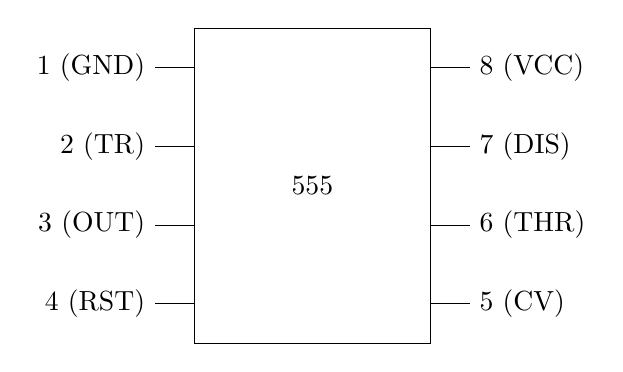
\begin{tikzpicture}
    \draw (0,0) rectangle (3,4);
    \node at (1.5, 2) {555};
    \foreach \y/\t in {3.5/8 (VCC), 2.5/7 (DIS), 1.5/6 (THR), 0.5/5 (CV)}
        \draw (3,\y) -- (3.5,\y) node[right] {\t};
    \foreach \y/\t in {3.5/1 (GND), 2.5/2 (TR), 1.5/3 (OUT), 0.5/4 (RST)}
        \draw (0,\y) -- (-0.5,\y) node[left] {\t};
\end{tikzpicture}
\end{center}

\textbf{Monostable Circuit \& Waveforms:}

\begin{center}
\begin{circuitikz}[american, scale=0.8, transform shape]
    % 555 Block inside
    \draw (0,0) rectangle (4,4);
    \node at (2,3.5) {IC 555};
    
    % External R-C
    \draw (2,4) -- (2,5) node[vcc] {$V_{CC}$};
    \draw (0,3) node[left] {Discharge (7)} -- (-1,3) to[R, l=$R$] (-1,5) -- (2,5);
    \draw (0,2) node[left] {Threshold (6)} -- (-1,2) -- (-1,3); % 6 shorted to 7? No!! Monostable: 6&7 connected.
    \draw (-1,2) to[C, l=$C$] (-1,0) node[ground] {};
    
    % Trigger
    \draw (0,1) node[left] {Trigger (2)} -- (-2,1) node[left] {Trig Input};
    
    % Output
    \draw (4,2) node[right] {Output (3)} -- (5,2) node[right] {$V_{out}$};
    
    % Ground
    \draw (2,0) -- (2,-0.5) node[ground] {};
    
    % Waveforms
    \begin{scope}[shift={(6,0)}]
        \draw[->] (0,0) -- (4,0) node[right] {$t$};
        \draw[->] (0,2.5) -- (0,3.5) node[above] {$V$};
        
        % Trigger
        \draw[blue] (0,3) -- (0.5,3) -- (0.5,1) -- (1,1) -- (1,3) -- (4,3);
        \node[blue, right] at (4,3) {Trigger};
        
        % Capacitor
        \draw[green!60!black] (0,0) -- (1,0) to[out=45, in=210] (3,2) -- (3,0) -- (4,0);
        \node[green!60!black, right] at (4,1) {$V_C$};
        
        % Output
        \draw[red] (0,0) -- (1,0) -- (1,2) -- (3,2) -- (3,0) -- (4,0);
        \node[red, right] at (4,2) {$V_{out}$};
        
        \draw[<->] (1,-0.5) -- (3,-0.5) node[midway, below] {$T = 1.1 RC$};
    \end{scope}
\end{circuitikz}
\end{center}

\begin{itemize}
    \item \textbf{Operation}: Trigger (Pin 2) low pulse starts timing cycle. Output goes high. Capacitor charges via R.
    \item \textbf{End of Cycle}: When $V_C = 2/3 V_{CC}$, output goes low, capacitor discharges.
    \item \textbf{Pulse Width}: $T = 1.1 \times R \times C$ seconds.
\end{itemize}

\begin{mnemonicbox}
"TIMER" - "Triggered Input Makes Extended Response"
\end{mnemonicbox}
\end{solutionbox}
\questionmarks{5(a)}{3}{Draw block diagram of SMPS and give its applications.}

\begin{solutionbox}
Switch Mode Power Supply (SMPS) uses switching elements for efficient power conversion.

\textbf{Block Diagram:}

\begin{center}
\begin{tikzpicture}[gtu block]
    \node [draw, rectangle] (ac) {AC Input};
    \node [draw, rectangle, right=0.5cm of ac] (rect1) {Rectifier \& Filter};
    \node [draw, rectangle, below=1cm of rect1] (switch) {Switching Circuit};
    \node [draw, rectangle, right=0.5cm of switch] (trans) {Transformer};
    \node [draw, rectangle, right=0.5cm of trans] (rect2) {Rectifier \& Filter};
    \node [draw, rectangle, above=1cm of rect2] (out) {Output};
    
    \draw [gtu arrow] (ac) -- (rect1);
    \draw [gtu arrow] (rect1) -- (switch);
    \draw [gtu arrow] (switch) -- (trans);
    \draw [gtu arrow] (trans) -- (rect2);
    \draw [gtu arrow] (rect2) -- (out);
    
    % Feedback
    \node [draw, rectangle, below=1cm of switch] (pwm) {PWM Control};
    \draw [gtu arrow] (out.east) -- ++(0.5,0) |- (pwm.east);
    \draw [gtu arrow] (pwm) -- (switch);
\end{tikzpicture}
\end{center}

\textbf{Applications:}
\begin{itemize}
    \item Computer power supplies (ATX)
    \item Mobile phone chargers
    \item TV power supplies
    \item LED lighting drivers
\end{itemize}

\begin{mnemonicbox}
"SAFE" - "Switching Achieves Filtered Energy"
\end{mnemonicbox}
\end{solutionbox}

\questionmarks{5(b)}{4}{Explain working of Regulated Power Supply with diagram.}

\begin{solutionbox}
Regulated power supply maintains constant output despite input or load variations.

\textbf{Block Diagram:}

\begin{center}
\begin{tikzpicture}[gtu block]
    \node [draw, rectangle] (ac) {AC Input};
    \node [draw, rectangle, right=0.5cm of ac] (trans) {Transformer};
    \node [draw, rectangle, right=0.5cm of trans] (rect) {Rectifier};
    \node [draw, rectangle, below=1cm of rect] (filt) {Filter};
    \node [draw, rectangle, left=0.5cm of filt] (reg) {Regulator};
    \node [draw, rectangle, left=0.5cm of reg] (load) {Load};
    
    \draw [gtu arrow] (ac) -- (trans);
    \draw [gtu arrow] (trans) -- (rect);
    \draw [gtu arrow] (rect) -- (filt);
    \draw [gtu arrow] (filt) -- (reg);
    \draw [gtu arrow] (reg) -- (load);
\end{tikzpicture}
\end{center}

\begin{itemize}
    \item \textbf{Transformer}: Steps down AC voltage to required level
    \item \textbf{Rectifier}: Converts AC to pulsating DC (diode bridge)
    \item \textbf{Filter}: Smooths DC ripple with capacitors
    \item \textbf{Regulator}: Stabilizes DC voltage (e.g., 7805, LM317)
\end{itemize}

\begin{mnemonicbox}
"TRFRO" - "Transform, Rectify, Filter, Regulate, Output"
\end{mnemonicbox}
\end{solutionbox}

\questionmarks{5(c)}{7}{Explain basic block diagram of OP-AMP with diagram.}

\begin{solutionbox}
Operational amplifier consists of four cascaded stages performing specific functions.

\textbf{Block Diagram:}

\begin{center}
\begin{tikzpicture}[gtu block]
    \node [draw, rectangle, align=center] (in) {Differential\\Input Stage};
    \node [draw, rectangle, align=center, right=0.5cm of in] (mid) {Intermediate\\Stage};
    \node [draw, rectangle, align=center, right=0.5cm of mid] (level) {Level\\Shifter};
    \node [draw, rectangle, align=center, right=0.5cm of level] (out) {Output\\Stage};
    
    \draw [gtu arrow] (in) -- (mid);
    \draw [gtu arrow] (mid) -- (level);
    \draw [gtu arrow] (level) -- (out);
    
    \node [below=0.5cm of mid] (const) {Constant Current Source};
    \draw [dashed] (const) -- (in);
    \draw [dashed] (const) -- (mid);
\end{tikzpicture}
\end{center}

\begin{itemize}
    \item \textbf{Differential Input Stage}: Provides high input impedance and CMRR (Dual Input Balanced Output)
    \item \textbf{Intermediate Stage}: Provides high voltage gain (Dual Input Unbalanced Output)
    \item \textbf{Level Shifter}: Shifts DC level to zero volts (Emitter Follower)
    \item \textbf{Output Stage}: Provides low output impedance and current drive (Push-Pull Amplifier)
\end{itemize}

\begin{mnemonicbox}
"DILO" - "Differential Input, Level shift, Output"
\end{mnemonicbox}
\end{solutionbox}

\vspace{0.5em}\centerline{\textbf{OR}}\questionmarks{5(a)}{3}{Explain adjustable voltage regulator using LM317 with diagram.}

\begin{solutionbox}
LM317 is a variable positive voltage regulator that adjusts output from 1.25V to 37V.

\textbf{Circuit Diagram:}

\begin{center}
\begin{circuitikz}[american, scale=1.0, transform shape]
    \draw (0,0) rectangle (2,1.5);
    \node at (1, 0.75) {LM317};
    \draw (-1, 1.25) to[short, o-] (0, 1.25) node[right] {IN};
    \draw (2, 1.25) to[short, -o] (4, 1.25) node[right] {$V_{out}$};
    \draw (2, 0.25) node[left] {ADJ} -- (2.5, 0.25) -- (2.5, -2) node[ground] {};
    
    \draw (2.5, 1.25) to[R, l=$R_1$] (2.5, 0.25); % R1 between OUT and ADJ
    \draw (2.5, 0.25) to[vR, l=$R_2$] (2.5, -2);
    
    \draw (-1, 1.25) to[C, l=$C_{in}$] (-1, 0) node[ground] {};
    \draw (4, 1.25) to[C, l=$C_{out}$] (4, 0) node[ground] {};
\end{circuitikz}
\end{center}

\begin{itemize}
    \item \textbf{Formula}: $V_{out} = 1.25V \times (1 + \frac{R_2}{R_1}) + I_{adj}R_2$ where $1.25V$ is reference voltage ($V_{ref}$)
    \item \textbf{Resistors}: $R_1$ sets reference current, $R_2$ adjusts output voltage
    \item \textbf{Protection}: Internal thermal overload and short circuit protection
\end{itemize}

\begin{mnemonicbox}
"AVR" - "Adjustable Voltage Regulation"
\end{mnemonicbox}
\end{solutionbox}

\questionmarks{5(b)}{4}{Give the difference between Fixed voltage regulator IC and Variable voltage regulator IC.}

\begin{solutionbox}
Comparison between fixed output regulators (like 78XX) and adjustable ones (like LM317).

\begin{center}
\captionof{table}{Fixed vs Variable Regulators}
\begin{tabulary}{\textwidth}{|L|L|L|}
\hline
\textbf{Parameter} & \textbf{Fixed Regulator} & \textbf{Variable Regulator} \\
\hline
Output Voltage & Preset (e.g., 5V, 12V) & Adjustable Range (e.g., 1.2V-37V) \\
\hline
Components & Minimum (2 Capacitors) & More (Resistors + Capacitors) \\
\hline
Flexibility & Low (Fixed application) & High (Universal application) \\
\hline
Examples & 7805, 7812, 7905 & LM317, LM337, LM723 \\
\hline
Cost & Generally Cheaper & Slightly Higher \\
\hline
Pin Config & In, Ground, Out & In, Adjust, Out \\
\hline
\end{tabulary}
\end{center}

\begin{mnemonicbox}
"FOCUS" - "Fixed Output Compared to User-Set"
\end{mnemonicbox}
\end{solutionbox}

\questionmarks{5(c)}{7}{List applications of OP-AMP. Explain working operation of D to A converter with circuit diagram using OP-AMP.}

\begin{solutionbox}
DAC converts digital binary input into equivalent analog voltage.

\textbf{Applications of OP-AMP:}
\begin{enumerate}
    \item Amplifiers (Inverting, Non-inverting, Differential)
    \item Filters (Active Low Pass, High Pass)
    \item Oscillators (Wein Bridge, Phase Shift)
    \item Comparators and Schmitt Triggers
    \item Mathematical Operations (Summing, Integrator, Differentiator)
\end{enumerate}

\textbf{R-2R Ladder DAC Circuit:}

\begin{center}
\begin{circuitikz}[american, scale=0.9, transform shape]
    \draw (0,0) node[op amp] (opamp) {};
    \draw (opamp.+) -- (-1, -0.5) node[ground] {};
    \draw (opamp.-) -- (-1, 0.5) -- (-1, 2) to[R, l=$R_f$] (1, 2) -| (opamp.out);
    \draw (opamp.out) to[short, -o] (2,0) node[right] {$V_{out}$};
    
    % Ladder
    \draw (-1, 0.5) -- (-2, 0.5); % Summing point
    \foreach \x in {0,1,2,3} {
        \draw (-2 - 2*\x, 0.5) -- (-2 - 2*\x - 2, 0.5); % Horizontal
        \draw (-2 - 2*\x, 0.5) to[R, l=$2R$] (-2 - 2*\x, -1.5) node[below] {$D_\x$}; % Vertical input
        \ifnum \x<3
            \draw (-2 - 2*\x - 2, 0.5) to[R, l=$R$] (-2 - 2*\x, 0.5); % Horizontal R (Wait, logic check)
        \fi
    }
    % Correct R-2R Ladder Layout logic:
    % From OpAmp (-) node, looks into ladder.
    % Ladder has series R, shunt 2R.
    % Terminating 2R at LSB end.
\end{circuitikz}

\begin{circuitikz}[american, scale=0.9, transform shape]
    \draw (0,0) node[op amp] (opamp) {};
    \draw (opamp.+) -- (-1, -0.5) node[ground] {};
    \draw (opamp.-) -- (-1, 0.5) -- (-1, 2) to[R, l=$3R$] (1, 2) -| (opamp.out);
    \draw (opamp.out) to[short, -o] (2,0) node[right] {$V_{out}$};

    % Ladder R-2R (4-bit)
    % Node 0 connects to opamp
    \draw (-1, 0.5) -- (-2, 0.5);
    \draw (-2, 0.5) to[R, l=$2R$] (-2, -1.5) node[below] {$b_3 (MSB)$};
    
    \draw (-2, 0.5) to[R, l=$R$] (-4, 0.5);
    \draw (-4, 0.5) to[R, l=$2R$] (-4, -1.5) node[below] {$b_2$};
    
    \draw (-4, 0.5) to[R, l=$R$] (-6, 0.5);
    \draw (-6, 0.5) to[R, l=$2R$] (-6, -1.5) node[below] {$b_1$};
    
    \draw (-6, 0.5) to[R, l=$R$] (-8, 0.5);
    \draw (-8, 0.5) to[R, l=$2R$] (-8, -1.5) node[below] {$b_0 (LSB)$};
    \draw (-8, 0.5) to[R, l=$2R$] (-10, 0.5) node[ground] {}; % Termination
    
\end{circuitikz}
\end{center}

\begin{itemize}
    \item \textbf{Principle}: Ladder network creates binary weighted currents
    \item \textbf{Output}: $V_{out} \propto -(b_3 2^{-1} + b_2 2^{-2} + b_1 2^{-3} + b_0 2^{-4}) V_{ref}$
    \item \textbf{Advantages}: Only two resistor values ($R, 2R$) needed, scalable
\end{itemize}

\begin{mnemonicbox}
"DART" - "Digital to Analog Resistor Translation"
\end{mnemonicbox}


\end{solutionbox}
\end{document}
